%!TEX root = ../dissertation.tex
\externaldocument{../frontmatter/abbr}
\externaldocument{./appendixA}
\externaldocument{./appendixB}
\begin{savequote}[75mm]
This is some random quote to start off the chapter.
\qauthor{Firstname lastname}
\end{savequote}
\chapter{Analisi dei requisiti}
\label{chap3}
\section{Casi d'uso}
\label{sec:usecase}
Di seguito verranno descritti i casi d'uso dell'applicazione, per quanto riguarda le funzionalità da me progettate; non verranno quindi tenute in considerazione eventuali funzionalità pre-esistenti che fossero parte dell'ecosistema a cui appartiene la piattaforma.

I casi d'uso verranno inoltre considerati per quanto concerne il \textit{back end} dell'applicazione, ovvero sulla base delle funzionalità realizzate per essere utilizzate dal \textit{front end}: eventuali aggiunte, quali la visualizzazione di messaggi di errore dettagliati o reindirizzamenti a pagine differenti della piattaforma web, verranno ignorate.

I casi d'uso verranno descritti mediante dei diagrammi \ref{itm:uml} che rappresentano le possibili interazioni tra gli \textbf{attori} ed il \textbf{sistema} dal punto di vista dei primi. È importante notare che il sistema, ovvero il \textit{back end} sviluppato, non viene utilizzato direttamente dagli utenti finali ma risponde a richieste di servizi esterni come il \textit{front end} (con l'eccezione degli utenti amministrativi, a cui viene fornita un'interfaccia di interazione ad-hoc): i casi d'uso verranno dunque trattati di conseguenza.

Di seguito verranno elencati solo i casi d'uso principali; per quelli secondari consultare l'\hyperref[sec:AppendixA]{appendice A}.
\subsection{Organizzazione dei casi d'uso}
\subsubsection{Attori}
\begin{itemize}
    \item \textbf{Utente non autenticato}: un utente che deve effettuare l'autenticazione per accedere alle funzionalità disponibili al suo ruolo;
    \item \textbf{Amministratore}: un utente autenticato con privilegi di accesso al pannello amministrativo.
    \item \textbf{Front end}: una istanza del \textit{front end} della piattaforma;
    \item \textbf{Gestionale laboratorio}: il software gestionale del laboratorio;
\end{itemize}
\vspace{-12pt}
\subsubsection{Struttura}
Per ogni caso d'uso, identificato da un codice univoco, vengono specificati gli attori coinvolti, lo scopo da raggiungere, le azioni previste e le condizioni del sistema prima e dopo tali azioni. I casi d'uso verranno descritti dalla seguente struttura:
\begin{itemize}
    \item Codice identificativo: \textbf{UC \{codice\_padre\}.\{codice\_figlio\}}
        \vspace{-5pt}
        \begin{itemize}
            \item \textbf{UC} indica che si tratta di un caso d'uso;
            \item \textbf{codice\_padre} identifica il caso d'uso principale a cui si fa riferimento;
            \item \textbf{codice\_figlio} identifica il sottocaso specifico;
        \end{itemize}
        \vspace{-5pt}
    \item Titolo
    \item Diagramma UML
    \item Attori
    \item Attori secondari, se presenti
    \item Scopo e descrizione
    \item Precondizioni
    \item Scenario principale
    \item Postcondizioni
    \item Inclusioni (se presenti)
    \item Estensioni (se presenti)
\end{itemize}
\vspace{-12pt}
\subsubsection{Casi d'uso generali}
Per una miglior suddivisione, le operazioni che avvengono sotto condizioni molto simili (principalmente quelle che possono essere richieste da un utente autenticato con un determinato ruolo) saranno raggruppate in dei casi d'uso di alto livello, d'ora in poi ``casi d'uso generali", identificati dalla lettera \textbf{G} prefissa al loro codice numerico. Tali casi d'uso servono solo per una miglior comprensione, quindi il loro codice non verrà considerato come \textbf{codice\_padre} nell'identificazione dei casi d'uso raggruppati.

\setlength{\parindent}{0cm}
\subsection{UC1: Autenticazione amministratore}
\label{sec:uc1}
\begin{figure}[h!]
    \centering
    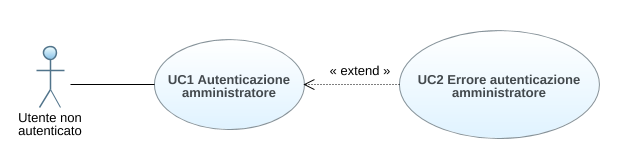
\includegraphics[width=.8\textwidth]{figures/uc/uc1gen.png}
    \caption[Diagramma UML per UC1 con estensioni]{Diagramma UML per UC1 con estensioni
    \label{fig:uc1}}
\end{figure}   
\begin{figure}[h!]
    \centering
    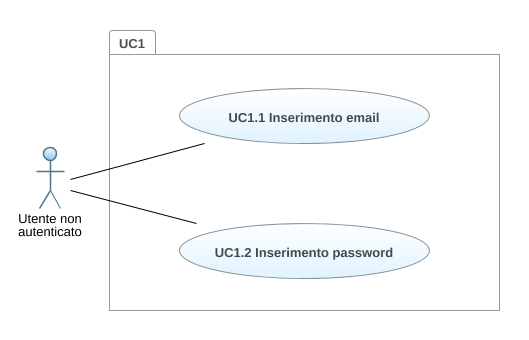
\includegraphics[height=6cm]{figures/uc/uc1.png}
    \caption[Diagramma UML per UC1 con sottocasi]{Diagramma UML per UC1 con sottocasi
    \label{fig:uc1}}
\end{figure}   
\textsc{\textsc{\textbf{Attori:}}} Utente non autenticato.\\
\textsc{\textbf{Scopo e descrizione:}} L'attore vuole effettuare la procedura di autenticazione al pannello di amministrazione.\\
\textsc{\textsc{\textbf{Precondizioni:}}} L'applicativo è stato avviato con successo e l'attore ha accesso alla pagina di autenticazione.\\
\textsc{\textbf{Scenario principale:}}
\begin{itemize}
    \item L'attore inserisce un indirizzo email valido (\hyperref[sec:uc11]{UC 1.1});
    \item L'attore inserisce la password associata a tale indirizzo email (\hyperref[sec:uc12]{UC 1.2});
    \item L'attore clicca sul pulsante di \textit{login}.
\end{itemize}
\textsc{\textbf{Postcondizioni:}} L'attore viene autenticato dal sistema e ha accesso al pannello di amministrazione.\\
\textsc{\textbf{Estensioni:}} L'attore non viene autenticato e visualizza un messaggio di errore (\hyperref[sec:uc2]UC2{}).

\subsection{UC2: Errore autenticazione amministratore}
\label{sec:uc2}
\textsc{\textbf{Attori:}} Utente non autenticato.\\
\textsc{\textbf{Scopo e descrizione:}} L'attore vuole effettuare la procedura di autenticazione al pannello di amministrazione.\\
\textsc{\textsc{\textbf{Precondizioni:}}} L'attore ha inserito le proprie credenziali negli appositi campi.\\
\textsc{\textbf{Scenario principale:}}
\begin{itemize}
    \item L'attore clicca sul pulsante di \textit{login};
    \item L'attore visualizza un messaggio di errore che lo informa che le credenziali non sono corrette.
\end{itemize}
\textsc{\textbf{Postcondizioni:}} L'attore non viene autenticato dal sistema e rimane nella pagina di autenticazione.

\subsection{UC3: Autenticazione front end}
\label{sec:uc3}
\label{sec:uc1}
\begin{figure}[h!]
    \centering
    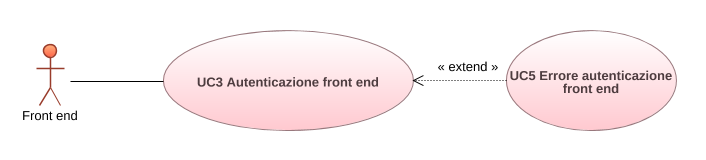
\includegraphics[width=\textwidth]{figures/uc/uc3gen.png}
    \caption[Diagramma UML per UC3]{Diagramma UML per UC3
    \label{fig:uc1}}
\end{figure}   
\textsc{\textbf{Attori:}} Front end.\\
\textsc{\textbf{Scopo e descrizione:}} L'attore vuole effettuare la procedura di autenticazione per un utente della piattaforma.\\
\textsc{\textsc{\textbf{Precondizioni:}}} L'applicativo è stato avviato con successo e l'attore è collegato correttamente al sistema.\\
\textsc{\textbf{Scenario principale:}} L'attore invia una richiesta di autenticazione contenente le credenziali di accesso di un utente autorizzato.\\
\textsc{\textbf{Postcondizioni:}} L'utente specificato dall'attore viene autenticato, e l'attore ha ricevuto in risposta i parametri della relativa sessione attiva.\\
\textsc{\textbf{Estensioni:}}  L'utente specificato dall'attore non viene riconosciuto, e l'attore ha ricevuto in risposta un messaggio di errore che lo informa che le credenziali non sono corrette (\hyperref[sec:UC5]{UC5}).

\subsection{UC4: Reset password per accesso alla piattaforma}
\label{sec:uc4}
\textsc{\textbf{Attori:}} Front end.\\
\textsc{\textbf{Scopo e descrizione:}} L'attore vuole effettuare la procedura di reset della password per un utente della piattaforma.\\
\textsc{\textsc{\textbf{Precondizioni:}}} L'applicativo è stato avviato con successo e l'attore è collegato correttamente al sistema.\\
\textsc{\textbf{Scenario principale:}} L'attore invia una richiesta di reset della password di accesso di un utente autorizzato.\\
\textsc{\textbf{Postcondizioni:}} È stata generata ed inviata all'utente una nuova password,e l'attore ha ricevuto una risposta di conferma del successo dell'operazione.

\subsection{UC5: Errore autenticazione front end}
\label{sec:UC5}
\textsc{\textbf{Attori:}} Front end.\\
\textsc{\textbf{Scopo e descrizione:}} L'attore vuole effettuare la procedura di autenticazione per un utente della piattaforma.\\
\textsc{\textsc{\textbf{Precondizioni:}}} L'attore ha inviato una richiesta di autenticazione al sistema.\\
\textsc{\textbf{Scenario principale:}} 
\begin{itemize}
    \item L'attore è in attesa di una risposta dal sistema;
    \item L'attore riceve in risposta un messaggio di errore che lo informa che le credenziali non sono corrette.
\end{itemize}
\textsc{\textbf{Postcondizioni:}} L'utente specificato dall'attore non viene riconosciuto e non ha ricevuto i dati di una sessione valida.

\subsection{UCG1: Operazioni amministrative}
\label{sec:ucg1}
\label{sec:uc1}    
Questo caso d'uso generale riassume le operazioni disponibili ad un utente autorizzato che abbia eseguito l'accesso al pannello di amministrazione. La maggior parte delle operazioni sui record sono identiche tra loro, e verranno quindi riportate in modo generalizzato; eventuali operazioni specifiche verranno contestualizzate nel proprio caso d'uso.
\begin{figure}[h!]
    \centering
    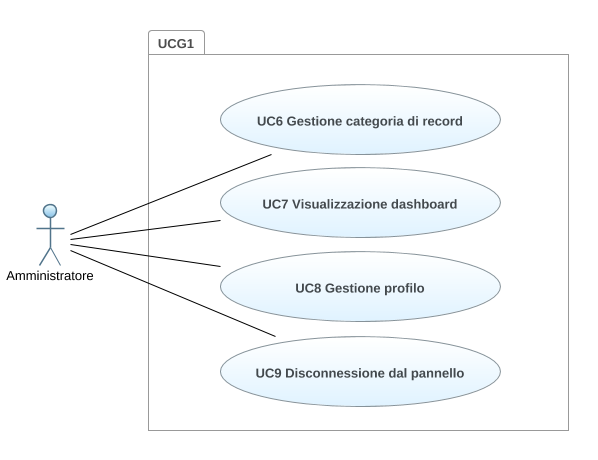
\includegraphics[width=.8\textwidth]{figures/uc/ucg1.png}
    \caption[Diagramma UML per UCG1]{Diagramma UML per UCG1
    \label{fig:ucg1}}
\end{figure}\\
\textsc{\textbf{Attori:}} Amministratore.\\
\textsc{\textbf{Scopo e descrizione:}} L'attore vuole eseguire operazioni di amministrazione della piattaforma.\\
\textsc{\textsc{\textbf{Precondizioni:}}} L'attore ha ottenuto l'accesso al pannello di amministrazione.\\
\textsc{\textbf{Scenario principale:}} 
\begin{itemize}
    \item L'attore visualizza e gestisce una categoria di record (\hyperref[sec:UC6]{UC6});
    \item L'attore visualizza la \textit{dashboard} (\hyperref[sec:UC7]{UC7});
    \item L'attore gestisce il proprio profilo (\hyperref[sec:UC8]{UC8});
    \item L'attore effettua la disconnessione dal pannello di amministrazione (\hyperref[sec:UC9]{UC9}).
\end{itemize}
\textsc{\textbf{Postcondizioni:}} L'attore ha correttamente portato a termine le operazioni desiderate.

\subsubsection{UC6: Gestione categoria di record}
\label{sec:UC6}
\begin{figure}[h!]
    \centering
    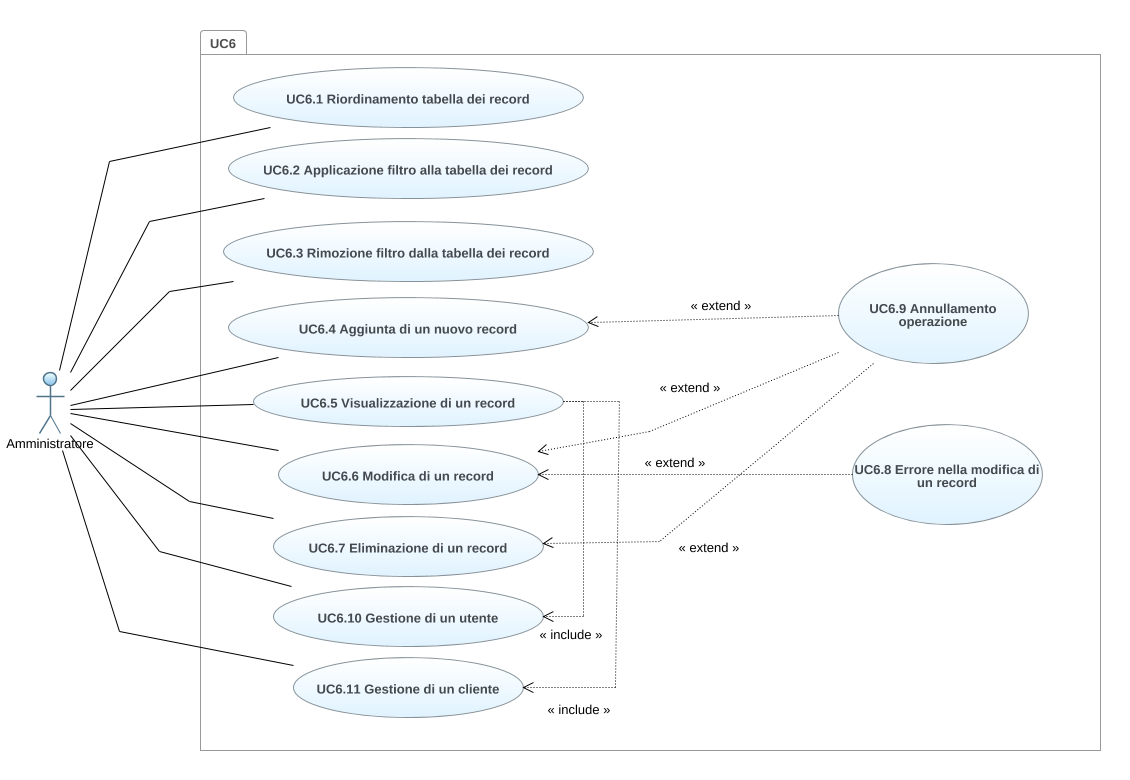
\includegraphics[width=\textwidth]{figures/uc/uc6.png}
    \caption[Diagramma UML per UC6]{Diagramma UML per UC6
    \label{fig:uc6}}
\end{figure}
\textsc{\textbf{Attori:}} Amministratore.\\
\textsc{\textbf{Scopo e descrizione:}} L'attore vuole gestire una particolare categoria di record.\\
\textsc{\textsc{\textbf{Precondizioni:}}} L'attore è nella \textit{dashboard} del pannello di amministrazione.\\
\textsc{\textbf{Scenario principale:}} 
\begin{itemize}
    \item L'attore seleziona una scheda associato alla categoria desiderata e visualizza la tabella dei record.
    \item L'attore modifica l'ordine della tabella dei record (\hyperref[sec:UC61]{UC6.1});
    \item L'attore applica un filtro alla tabella dei record (\hyperref[sec:UC62]{UC6.2});
    \item L'attore rimuove un filtro dalla tabella dei record (\hyperref[sec:UC63]{UC6.3});
    \item L'attore aggiunge un nuovo record (\hyperref[sec:UC64]{UC6.4});
    \item L'attore visualizza un record particolare (\hyperref[sec:UC65]{UC6.5});
    \item L'attore modifica un record particolare (\hyperref[sec:UC66]{UC6.6});
    \item L'attore elimina un record particolare (\hyperref[sec:UC67]{UC6.7});
    \item L'attore gestisce un utente (\hyperref[sec:UC610]{UC6.10}).
    \item L'attore gestisce un cliente (\hyperref[sec:UC611]{UC6.11}).
\end{itemize}
\textsc{\textbf{Postcondizioni:}} L'attore ha eseguito tutte le operazioni di gestione della categoria di record selezionata con successo.

\subsubsection{UC7: Visualizzazione dashboard}
\label{sec:UC7}
\textsc{\textbf{Attori:}} Amministratore.\\
\textsc{\textbf{Scopo e descrizione:}} L'attore vuole visualizzare la \textit{dashboard} del pannello di amministrazione.\\
\textsc{\textsc{\textbf{Precondizioni:}}} L'attore sta visualizzando una pagina diversa dalla \textit{dashboard}.\\
\textsc{\textbf{Scenario principale:}} L'attore seleziona la scheda ``Dashboard".\\
\textsc{\textbf{Postcondizioni:}} L'attore viene reindirizzato alla pagina della \textit{dashboard}.

\subsubsection{UC8: Gestione profilo}
\label{sec:UC8}
\textsc{\textbf{Attori:}} Amministratore.\\
\textsc{\textbf{Scopo e descrizione:}} L'attore vuole gestire il proprio profilo utente.\\
\textsc{\textsc{\textbf{Precondizioni:}}} L'attore ha accesso al pannello di amministrazione.\\
\textsc{\textbf{Scenario principale:}}
\begin{itemize}
    \item L'attore clicca sull'icona del profilo.
    \item L'attore visualizza il record relativo al proprio profilo (\hyperref[sec:UC65]{UC6.5})
\end{itemize}
\textsc{\textbf{Postcondizioni:}} L'attore ha gestito correttamente il proprio profilo.

\subsubsection{UC9: Disconnessione}
\label{sec:UC9}
\textsc{\textbf{Attori:}} Amministratore.\\
\textsc{\textbf{Scopo e descrizione:}} L'attore vuole disconnettersi dal pannello di amministrazione.\\
\textsc{\textsc{\textbf{Precondizioni:}}} L'attore ha accesso al pannello di amministrazione.\\
\textsc{\textbf{Scenario principale:}} L'attore clicca sull'icona di disconnessione.\\
\textsc{\textbf{Postcondizioni:}} L'attore viene correttamente disconnesso dal pannello di amministrazione.

\subsection{UCG2: Operazioni per utente ``pharmacy''}
\label{sec:UCG2}
Questo caso d'uso generale riassume le operazioni disponibili al \textit{front end} quando è attiva una sessione per un utente con ruolo di ``pharmacy''. Come anticipato, le operazioni vengono considerate non dal punto di vista dell'utente finale della piattaforma, cioè il farmacista o cliente che si interfaccia con il \textit{front end}, ma come richieste che l'istanza di \textit{front end} può effettuare alle \ref{itm:api} del servizio \textit{back end}. Non verranno, per questo motivo, quindi fatte distinzioni tra interazioni che verrebbero effettuate da un farmacista o da un cliente. Infine, va considerato implicito che ognuna delle seguenti operazioni è ristretta ai record del database resi visibili dalla sessione attiva (nella fattispecie i record associati alla farmacia a cui appartiene l'utente autenticato).
\begin{figure}[h!]
    \centering
    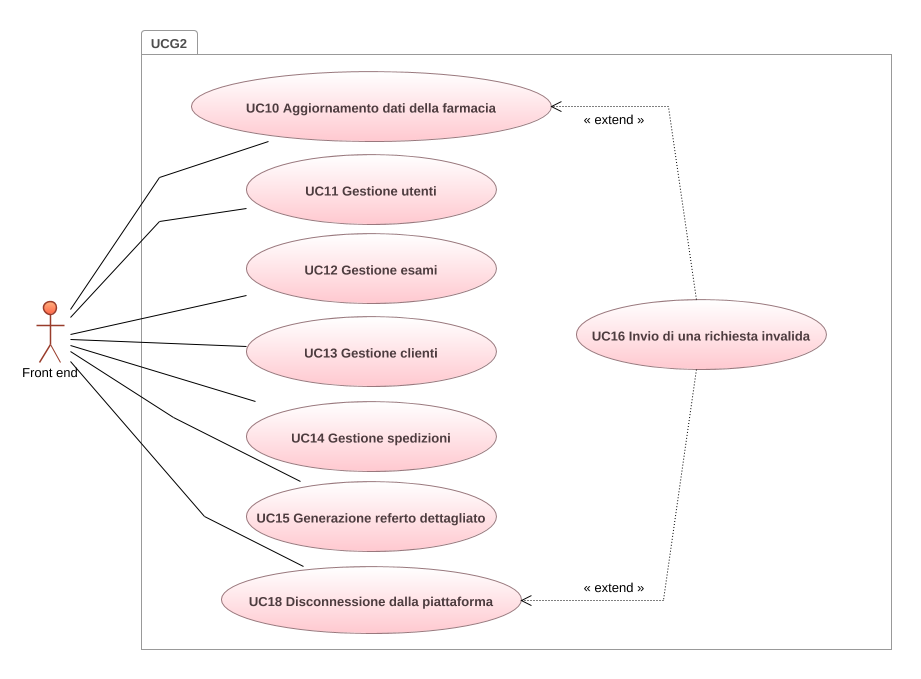
\includegraphics[width=\textwidth]{figures/uc/ucg2.png}
    \caption[Diagramma UML per UCG2]{Diagramma UML per UCG2
    \label{fig:ucg2}}
\end{figure}\\
\textsc{\textbf{Attori:}} Front end.\\
\textsc{\textbf{Scopo e descrizione:}} L'attore vuole eseguire operazioni permesse ad un utente con ruolo di ``pharmacy''.\\
\textsc{\textsc{\textbf{Precondizioni:}}} L'attore è collegato al sistema e possiede una sessione attiva per un utente con ruolo ``pharmacy''.\\
\textsc{\textbf{Scenario principale:}} 
\begin{itemize}
    \item L'attore modifica i dati della farmacia (\hyperref[sec:UC10]{UC10});
    \item L'attore gestisce gli utenti con ruolo ``pharmacy'' (\hyperref[sec:UC11]{UC11});
    \item L'attore gestisce gli esami (\hyperref[sec:UC12]{UC12});
    \item L'attore gestisce i clienti (\hyperref[sec:UC13]{UC13});
    \item L'attore gestisce le spedizioni (\hyperref[sec:UC14]{UC14});
    \item L'attore visualizza il referto dettagliato per un esame (\hyperref[sec:UC15]{UC15});
    \item L'attore effettua la disconnessione dalla piattaforma (\hyperref[sec:UC18]{UC18}).
\end{itemize}
\textsc{\textbf{Postcondizioni:}} L'attore ha correttamente portato a termine le operazioni desiderate.

\subsubsection{UC10: Aggiornamento dati della farmacia}
\label{sec:UC10}
\textsc{\textbf{Attori:}} Front end.\\
\textsc{\textbf{Scopo e descrizione:}} L'attore vuole aggiornare i dati della farmacia corrente.\\
\textsc{\textsc{\textbf{Precondizioni:}}} L'attore è collegato al sistema e possiede una sessione attiva per un utente con ruolo ``pharmacy''.\\
\textsc{\textbf{Scenario principale:}} L'attore invia una richiesta di aggiornamento del record della farmacia con i nuovi dati, potenzialmente allegando un'immagine da sostituire al logo corrente.\\
\textsc{\textbf{Postcondizioni:}} Il record corrispondente alla farmacia viene aggiornato e l'attore ha ricevuto una risposta che conferma il successo dell'operazione.\\
\textsc{\textbf{Estensioni:}} L'attore invia una richiesta non valida (\hyperref[sec:UC16]{UC16}).


\subsubsection{UC11: Gestione utenti}
\label{sec:UC11}
\textsc{\textbf{Attori:}} Front end.\\
\textsc{\textbf{Scopo e descrizione:}} L'attore vuole gestire gli altri utenti con ruolo ``pharmacy'' appartenenti alla farmacia corrente.\\
\textsc{\textsc{\textbf{Precondizioni:}}} L'attore è collegato al sistema e possiede una sessione attiva per un utente con ruolo ``pharmacy''.\\
\textsc{\textbf{Scenario principale:}}
\begin{itemize}
    \item L'attore richiede la lista degli utenti (\hyperref[sec:UC111]{UC11.1});
    \item L'attore richiede i dati di un utente (\hyperref[sec:UC112]{UC11.2});
    \item L'attore richiede il reset della password di un utente (\hyperref[sec:UC113]{UC11.3});
    \item L'attore imposta una nuova password per un utente  (\hyperref[sec:UC114]{UC11.4});
    \item L'attore crea un utente (\hyperref[sec:UC115]{UC11.5});
    \item L'attore elimina un utente (\hyperref[sec:UC116]{UC11.6});
    \item L'attore aggiorna i dati di un utente (\hyperref[sec:UC117]{UC11.7}).
\end{itemize}
\textsc{\textbf{Postcondizioni:}} L'attore ha portato a termine con successo le operazioni di gestione degli utenti.

\subsubsection{UC12: Gestione esami}
\label{sec:UC12}
\textsc{\textbf{Attori:}} Front end.\\
\textsc{\textbf{Scopo e descrizione:}} L'attore vuole gestire gli altri utenti con ruolo ``pharmacy'' appartenenti alla farmacia corrente.\\
\textsc{\textsc{\textbf{Precondizioni:}}} L'attore è collegato al sistema e possiede una sessione attiva per un utente con ruolo ``pharmacy''.\\
\textsc{\textbf{Scenario principale:}}
\begin{itemize}
    \item L'attore richiede lo storico degli esami (\hyperref[sec:UC121]{UC12.1});
    \item L'attore richiede lo storico degli esami in base allo stato di avanzamento (\hyperref[sec:UC122]{UC12.2});
    \item L'attore richiede i dati un esame (\hyperref[sec:UC123]{UC12.3});
    \item L'attore richiede i dati di esame in base al codice campione (\hyperref[sec:UC124]{UC12.4});
    \item L'attore crea un nuovo esame (\hyperref[sec:UC125]{UC12.5});
    \item L'attore rimuove un esame (\hyperref[sec:UC126]{UC12.6});
    \item L'attore aggiorna i dati di un esame (\hyperref[sec:UC127]{UC12.7});
    \item L'attore aggiorna le risposte al questionario di un'esame (\hyperref[sec:UC128]{UC12.8}).
\end{itemize}
\textsc{\textbf{Postcondizioni:}} L'attore ha portato a termine con successo le operazioni di gestione degli utenti.

\subsubsection{UC13: Gestione clienti}
\label{sec:UC13}
\textsc{\textbf{Attori:}} Front end.\\
\textsc{\textbf{Scopo e descrizione:}} L'attore vuole gestire i clienti appartenenti alla farmacia corrente.\\
\textsc{\textsc{\textbf{Precondizioni:}}} L'attore è collegato al sistema e possiede una sessione attiva per un utente con ruolo ``pharmacy''.\\
\textsc{\textbf{Scenario principale:}}
\begin{itemize}
    \item L'attore richiede il registro dei clienti (\hyperref[sec:UC131]{UC13.1});
    \item L'attore richiede i dati di un cliente (\hyperref[sec:UC132]{UC13.2});
    \item L'attore crea un cliente (\hyperref[sec:UC133]{UC13.3});
    \item L'attore elimina un cliente (\hyperref[sec:UC134]{UC13.4});
    \item L'attore aggiorna i dati di un cliente (\hyperref[sec:UC135]{UC13.5});
    \item L'attore invia il codice per accettare la \textit{privacy policy} ad un cliente (\hyperref[sec:UC136]{UC13.6});
    \item L'attore verifica l'accettazione della \textit{privacy policy} per un cliente (\hyperref[sec:UC137]{UC13.7});
    \item L'attore effettua il caricamento di un modulo per il consenso alla \textit{privacy policy} firmato da un cliente (\hyperref[sec:UC138]{UC13.8}).
\end{itemize}
\textsc{\textbf{Postcondizioni:}} L'attore ha portato a termine con successo le operazioni di gestione dei clienti.

\subsubsection{UC14: Gestione spedizioni}
\label{sec:UC14}
\textsc{\textbf{Attori:}} Front end.\\
\textsc{\textbf{Scopo e descrizione:}} L'attore vuole gestire le spedizioni per la farmacia corrente.\\
\textsc{\textsc{\textbf{Precondizioni:}}} L'attore è collegato al sistema e possiede una sessione attiva per un utente con ruolo ``pharmacy''.\\
\textsc{\textbf{Scenario principale:}}
\begin{itemize}
    \item L'attore visualizza la lista delle spedizioni (\hyperref[sec:UC141]{UC14.1});
    \item L'attore visualizza una spedizione (\hyperref[sec:UC142]{UC14.2});
    \item L'attore crea una spedizione (\hyperref[sec:UC143]{UC14.3});
    \item L'attore elimina una spedizione (\hyperref[sec:UC144]{UC14.4});
    \item L'attore modifica i dati di una spedizione (\hyperref[sec:UC145]{UC14.5});
    \item L'attore visualizza la lettera di vettura per una spedizione (\hyperref[sec:UC146]{UC14.6});
    \item L'attore prenota il ritiro di una spedizione (\hyperref[sec:UC147]{UC14.7}).
\end{itemize}
\textsc{\textbf{Postcondizioni:}} L'attore ha portato a termine con successo le operazioni di gestione delle spedizioni.

\subsubsection{UC15: Generazione referto dettagliato}
\label{sec:UC15}
\textsc{\textbf{Attori:}} Front end.\\
\textsc{\textbf{Scopo e descrizione:}} L'attore vuole visualizzare il referto di un esame, completo delle informazioni specifiche risultate dall'analisi e delle informazioni personali del cliente.\\
\textsc{\textsc{\textbf{Precondizioni:}}} L'attore è collegato al sistema ed l'esame desiderato è arrivato correttamente in stato \textbf{final}.\\
\textsc{\textbf{Scenario principale:}}
\begin{itemize}
    \item L'attore richiede la visualizzazione del referto, fornendo il codice identificativo interno dell'esame cui è associato;
    \item Il sistema processa il file PDF del referto inviato dal laboratorio aggiungendo la diagnosi del gastroenterologo, la tabella della dieta e le generalità del paziente;
    \item L'attore riceve dal sistema il referto generato.
\end{itemize}
\textsc{\textbf{Postcondizioni:}} L'attore ha visualizzato correttamente il referto specifico.\\
\textsc{\textbf{Estensioni:}} L'attore invia una richiesta non valida (\hyperref[sec:UC16]{UC16}).

\subsubsection{UC16: Invio di una richiesta invalida}
\label{sec:UC16}
\textsc{\textbf{Attori:}} Front end.\\
\textsc{\textbf{Scopo e descrizione:}} L'attore vuole inviare una richiesta al sistema.\\
\textsc{\textsc{\textbf{Precondizioni:}}} L'attore è collegato al sistema e possiede una richiesta contenente dati non validi.\\
\textsc{\textbf{Scenario principale:}}
\begin{itemize}
    \item L'attore invia la richiesta con dati non validi;
    \item L'attore riceve un messaggio di errore che descrive la violazione commessa.
\end{itemize}
\textsc{\textbf{Postcondizioni:}} La richiesta dell'attore viene rifiutata e l'attore ha ricevuto un messaggio di errore appropriato.

\subsubsection{UC17: Superamento tentativi di invio del codice OTP}
\label{sec:UC17}
\textsc{\textbf{Attori:}} Front end.\\
\textsc{\textbf{Scopo e descrizione:}} L'attore vuole inviare il codice per l'accettazione della privacy policy ad un cliente della farmacia corrente.\\
\textsc{\textsc{\textbf{Precondizioni:}}} Sono già stati effettuati 3 tentativi nelle ultime 24 ore.\\
\textsc{\textbf{Scenario principale:}}
\begin{itemize}
    \item L'attore richiede l'invio del codice;
    \item L'attore riceve un messaggio di errore che lo informa del superamento del numero massimo di tentativi per la giornata.
\end{itemize}
\textsc{\textbf{Postcondizioni:}} La richiesta dell'attore viene rifiutata e l'attore ha ricevuto un messaggio di errore appropriato.

\subsubsection{UC18: Disconnessione dalla piattaforma}
\label{sec:UC18}
\textsc{\textbf{Attori:}} Front end.\\
\textsc{\textbf{Scopo e descrizione:}} L'attore vuole disconnettersi dalla piattaforma.\\
\textsc{\textsc{\textbf{Precondizioni:}}} L'attore è collegato al sistema e possiede una sessione attiva.\\
\textsc{\textbf{Scenario principale:}}
\begin{itemize}
    \item L'attore richiede la disconnessione dalla piattaforma;
    \item Il sistema invalida i parametri della sessione corrente.
\end{itemize}
\textsc{\textbf{Postcondizioni:}} L'attore viene disconnesso correttamente e il sistema non accetta più richieste con i parametri della sessione invalidata.

\subsection{UCG3: Operazioni per utente ``gastroenterologist''}
\label{sec:UCG3}
Questo caso d'uso generale riassume le operazioni disponibili al \textit{front end} quando è attiva una sessione per un utente con ruolo di ``gastroenterologist''. Valgono le stesse considerazioni fatte per \hyperref[sec:UCG2]{UCG2}, con l'eccezione dei record disponibili: nella descrizione dei seguenti casi d'uso le operazioni non sono ristrette ai record associati ad una farmacia, ma escludono rigorosamente i dati personali dei clienti.\\
\textsc{\textbf{Attori:}} Front end.\\
\textsc{\textbf{Scopo e descrizione:}} L'attore vuole eseguire operazioni permesse ad un utente con ruolo di ``gastroenterologist''.\\
\textsc{\textbf{Precondizioni:}} L'attore è collegato al sistema e possiede una sessione attiva per un utente con ruolo ``gastroenterologist''.\\
\textsc{\textbf{Scenario principale:}} 
\begin{itemize}
    \item L'attore richiede la lista di esami in attesa di diagnosi (\hyperref[sec:UC19]{UC19});
    \item L'attore richiede i dati di un esame in attesa di diagnosi (\hyperref[sec:UC20]{UC20});
    \item L'attore inserisce una diagnosi per un esame (\hyperref[sec:UC21]{UC21});
    \item L'attore inserisce la tabella della dieta per un esame (\hyperref[sec:UC22]{UC22});
    \item L'attore visualizza il referto dettagliato anonimo per un esame (\hyperref[sec:UC23]{UC23});
    \item L'attore effettua la disconnessione dalla piattaforma (\hyperref[sec:UC18]{UC18}).
\end{itemize}
\textsc{\textbf{Postcondizioni:}} L'attore ha correttamente portato a termine le operazioni desiderate.

\subsubsection{UC19: Richiesta lista esami in attesa di diagnosi}
\label{sec:UC19}
\textsc{\textbf{Attori:}} Front end.\\
\textsc{\textbf{Scopo e descrizione:}} L'attore vuole ottenere la lista degli esami per cui è disponibile il referto delle analisi e sono quindi in attesa di diagnosi.\\
\textsc{\textsc{\textbf{Precondizioni:}}} L'attore è collegato al sistema e possiede una sessione attiva per un utente con ruolo ``gastroenterologist''.\\
\textsc{\textbf{Scenario principale:}} L'attore invia una richiesta per ottenere la lista di esami desiderata.\\
\textsc{\textbf{Postcondizioni:}} L'attore ha ricevuto correttamente i dati richiesti al sistema.\\
\textsc{\textbf{Estensioni:}} L'attore invia una richiesta non valida (\hyperref[sec:UC16]{UC16}).

\subsubsection{UC20: Richiesta informazioni per un esame in attesa di diagnosi}
\label{sec:UC20}
\textsc{\textbf{Attori:}} Front end.\\
\textsc{\textbf{Scopo e descrizione:}} L'attore vuole ottenere i dati di un esame  per cui è disponibile il referto delle analisi ed è quindi in attesa di diagnosi.\\
\textsc{\textsc{\textbf{Precondizioni:}}} L'attore è collegato al sistema e possiede una sessione attiva per un utente con ruolo ``gastroenterologist''.\\
\textsc{\textbf{Scenario principale:}}  L'attore invia una richiesta per ottenere l'esame desiderato, fornendone il codice identificativo interno .\\
\textsc{\textbf{Postcondizioni:}} L'attore ha ricevuto correttamente i dati richiesti al sistema.\\
\textsc{\textbf{Estensioni:}} L'attore invia una richiesta non valida (\hyperref[sec:UC16]{UC16}).

\subsubsection{UC21: Inserimento diagnosi per un esame}
\label{sec:UC21}
\textsc{\textbf{Attori:}} Front end.\\
\textsc{\textbf{Scopo e descrizione:}} L'attore vuole inserire una diagnosi per un esame.\\
\textsc{\textsc{\textbf{Precondizioni:}}} L'attore è collegato al sistema e possiede una sessione attiva per un utente con ruolo ``gastroenterologist'', l'esame rientra tra quelli visibili.\\
\textsc{\textbf{Scenario principale:}}  L'attore invia una richiesta di inserimento della diagnosi per l'esame desiderato contenente le informazioni generali e specifiche della diagnosi, fornendo il codice identificativo interno dell'esame.\\
\textsc{\textbf{Postcondizioni:}} Il sistema ha registrato correttamente la diagnosi e l'attore ha ricevuto una risposta che conferma il successo dell'operazione.\\
\textsc{\textbf{Estensioni:}} L'attore invia una richiesta non valida (\hyperref[sec:UC16]{UC16}).

\subsubsection{UC22: Inserimento tabella della dieta}
\label{sec:UC22}
\textsc{\textbf{Attori:}} Front end.\\
\textsc{\textbf{Scopo e descrizione:}} L'attore vuole inserire la tabella della dieta associata ad un esame.\\
\textsc{\textsc{\textbf{Precondizioni:}}} L'attore è collegato al sistema e possiede una sessione attiva per un utente con ruolo ``gastroenterologist'', l'esame rientra tra quelli visibili.\\
\textsc{\textbf{Scenario principale:}}  L'attore invia una richiesta di inserimento della tabella della dieta per l'esame desiderato, fornendo il codice identificativo interno dell'esame.\\
\textsc{\textbf{Postcondizioni:}} Il sistema ha registrato correttamente la tabella della dieta e l'attore ha ricevuto una risposta che conferma il successo dell'operazione.\\
\textsc{\textbf{Estensioni:}} L'attore invia una richiesta non valida (\hyperref[sec:UC16]{UC16}).

\subsubsection{UC23: Generazione referto dettagliato anonimo}
\label{sec:UC23}
\textsc{\textbf{Attori:}} Front end.\\
\textsc{\textbf{Scopo e descrizione:}} L'attore vuole visualizzare il referto di un esame, completo delle informazioni specifiche risultate dall'analisi.\\
\textsc{\textsc{\textbf{Precondizioni:}}} L'attore è collegato al sistema e possiede una sessione attiva per un utente con ruolo ``gastroenterologist'' o ``bmr'', l'esame rientra tra quelli visibili.\\
\textsc{\textbf{Scenario principale:}}
\begin{itemize}
    \item L'attore richiede la visualizzazione del referto, fornendo il codice identificativo interno dell'esame cui è associato;
    \item Il sistema processa il file PDF del referto inviato dal laboratorio aggiungendo la diagnosi del gastroenterologo e la tabella della dieta;
    \item L'attore riceve dal sistema il referto generato.
\end{itemize}
\textsc{\textbf{Postcondizioni:}} L'attore ha visualizzato correttamente il referto specifico.\\
\textsc{\textbf{Estensioni:}} L'attore invia una richiesta non valida (\hyperref[sec:UC16]{UC16}).

\subsection{UCG4: Operazioni per utente ``bmr''}
\label{sec:UCG4}
Questo caso d'uso generale riassume le operazioni disponibili al \textit{front end} quando è attiva una sessione per un utente con ruolo di ``bmr'' (supervisore del laboratorio). Valgono le stesse considerazioni fatte per \hyperref[sec:UCG3]{UCG3}.
\textsc{\textbf{Attori:}} Front end.\\
\textsc{\textbf{Scopo e descrizione:}} L'attore vuole eseguire operazioni permesse ad un utente con ruolo di ``bmr''.\\
\textsc{\textbf{Precondizioni:}} L'attore è collegato al sistema e possiede una sessione attiva per un utente con ruolo ``bmr''.\\
\textsc{\textbf{Scenario principale:}} 
\begin{itemize}
    \item L'attore richiede la lista di esami per cui è stata emessa una diagnosi (\hyperref[sec:UC24]{UC24});
    \item L'attore richiede i dati di un esame per cui è stata emessa una diagnosi (\hyperref[sec:UC25]{UC25});
    \item L'attore aggiorna una diagnosi per un esame (\hyperref[sec:UC26]{UC26});
    \item L'attore aggiorna la tabella della dieta per un esame (\hyperref[sec:UC27]{UC27});
    \item L'attore visualizza il referto dettagliato anonimo per un esame (\hyperref[sec:UC23]{UC23});
    \item L'attore effettua la disconnessione dalla piattaforma (\hyperref[sec:UC18]{UC18}).
\end{itemize}
\textsc{\textbf{Postcondizioni:}} L'attore ha correttamente portato a termine le operazioni desiderate.

\subsubsection{UC24: Richiesta lista esami con diagnosi}
\label{sec:UC24}
\textsc{\textbf{Attori:}} Front end.\\
\textsc{\textbf{Scopo e descrizione:}} L'attore vuole ottenere la lista degli esami per cui è stata emessa una diagnosi.\\
\textsc{\textsc{\textbf{Precondizioni:}}} L'attore è collegato al sistema e possiede una sessione attiva per un utente con ruolo ``bmr''.\\
\textsc{\textbf{Scenario principale:}} L'attore invia una richiesta per ottenere la lista di esami desiderata.\\
\textsc{\textbf{Postcondizioni:}} L'attore ha ricevuto correttamente i dati richiesti al sistema.\\
\textsc{\textbf{Estensioni:}} L'attore invia una richiesta non valida (\hyperref[sec:UC16]{UC16}).

\subsubsection{UC25: Richiesta informazioni esame con diagnosi}
\label{sec:UC25}
\textsc{\textbf{Attori:}} Front end.\\
\textsc{\textbf{Scopo e descrizione:}} L'attore vuole ottenere i dati di un esame per cui è stata emessa una diagnosi.\\
\textsc{\textsc{\textbf{Precondizioni:}}} L'attore è collegato al sistema e possiede una sessione attiva per un utente con ruolo ``gastroenterologist''.\\
\textsc{\textbf{Scenario principale:}}  L'attore invia una richiesta per ottenere l'esame desiderato, fornendone il codice identificativo interno .\\
\textsc{\textbf{Postcondizioni:}} L'attore ha ricevuto correttamente i dati richiesti al sistema.\\
\textsc{\textbf{Estensioni:}} L'attore invia una richiesta non valida (\hyperref[sec:UC16]{UC16}).

\subsubsection{UC26: Aggiornamento diagnosi per un esame}
\label{sec:UC26}
\textsc{\textbf{Attori:}} Front end.\\
\textsc{\textbf{Scopo e descrizione:}} L'attore vuole modificare la diagnosi emessa per un esame.\\
\textsc{\textsc{\textbf{Precondizioni:}}} L'attore è collegato al sistema e possiede una sessione attiva per un utente con ruolo ``bmr'', l'esame rientra tra quelli visibili.\\
\textsc{\textbf{Scenario principale:}}  L'attore invia una richiesta di modifica della diagnosi per l'esame desiderato contenente le nuove informazioni generali e specifiche della diagnosi, fornendo il codice identificativo interno dell'esame.\\
\textsc{\textbf{Postcondizioni:}} Il sistema ha aggiornato correttamente la diagnosi e l'attore ha ricevuto una risposta che conferma il successo dell'operazione.\\
\textsc{\textbf{Estensioni:}} L'attore invia una richiesta non valida (\hyperref[sec:UC16]{UC16}).

\subsubsection{UC27: Aggiornamento tabella della dieta}
\label{sec:UC27}
\textsc{\textbf{Attori:}} Front end.\\
\textsc{\textbf{Scopo e descrizione:}} L'attore vuole aggiornare la tabella della dieta associata ad un esame.\\
\textsc{\textsc{\textbf{Precondizioni:}}} L'attore è collegato al sistema e possiede una sessione attiva per un utente con ruolo ``bmr'', l'esame rientra tra quelli visibili.\\
\textsc{\textbf{Scenario principale:}}  L'attore invia una richiesta di modifica della tabella della dieta per l'esame desiderato, fornendo il codice identificativo interno dell'esame.\\
\textsc{\textbf{Postcondizioni:}} Il sistema ha aggiornato correttamente la tabella della dieta e l'attore ha ricevuto una risposta che conferma il successo dell'operazione.\\
\textsc{\textbf{Estensioni:}} L'attore invia una richiesta non valida (\hyperref[sec:UC16]{UC16}).

\subsection{UCG5: Operazioni per il gestionale del laboratorio}
\label{sec:UCG5}
Questo caso d'uso generale riassume le operazioni disponibili al software gestionale del laboratorio attraverso gli appositi \textit{endpoint} \ref{itm:http}. Si prevede che le richieste \ref{itm:http} contengano, nella sezione \textit{header}, le credenziali necessarie per l'autenticazione tramite HMAC.\\ 
\textsc{\textbf{Attori:}} Gestionale laboratorio.\\
\textsc{\textbf{Scopo e descrizione:}} L'attore vuole eseguire operazioni rese disponibili dagli \textit{endpoint} esposti.\\
\textsc{\textbf{Precondizioni:}} L'attore ha accesso agli \textit{endpoint} forniti dal sistema e possiede le credenziali necessarie per l'autenticazione HMAC.\\
\textsc{\textbf{Scenario principale:}} 
\begin{itemize}
    \item L'attore richiede la lista di esami il cui campione è stato raccolto (\hyperref[sec:UC28]{UC28});
    \item L'attore richiede i dati di un esame (\hyperref[sec:UC29]{UC29});
    \item L'attore aggiorna lo stato di avanzamento di un esame (\hyperref[sec:UC30]{UC30});
    \item L'attore rifiuta il campione per un esame (\hyperref[sec:UC31]{UC31});
    \item L'attore carica il referto delle analisi (\hyperref[sec:UC32]{UC32}).
    \item L'attore richiede il referto dettagliato anonimo per un esame (\hyperref[sec:UC33]{UC33})
\end{itemize}
\textsc{\textbf{Postcondizioni:}} L'attore ha correttamente portato a termine le operazioni desiderate.

\subsubsection{UC28: Richiesta lista esami con campione}
\label{sec:UC28}
\textsc{\textbf{Attori:}} Gestionale laboratorio.\\
\textsc{\textbf{Scopo e descrizione:}} L'attore vuole ottenere la lista degli esami il cui campione è stato raccolto, compresi quelli il cui iter di avanzamento è stato completato.\\
\textsc{\textsc{\textbf{Precondizioni:}}} L'attore ha accesso all'\textit{endpoint} corrispondente e ha autenticato correttamente la richiesta.\\
\textsc{\textbf{Scenario principale:}}  L'attore invia la richiesta \ref{itm:http} di sincronizzazione della lista degli esami all'\textit{endpoint} appropriato.\\
\textsc{\textbf{Postcondizioni:}} L'attore ha ricevuto una risposta contenente i dati richiesti in formato \ref{itm:json}.\\
\textsc{\textbf{Estensioni:}} L'attore invia una richiesta non valida e ottiene una risposta che segnala l'errore (\hyperref[sec:UC34]{UC34}).

\subsubsection{UC29: Richiesta dati di un esame}
\label{sec:UC29}
\textsc{\textbf{Attori:}} Gestionale laboratorio.\\
\textsc{\textbf{Scopo e descrizione:}} L'attore vuole ottenere i dati di un esame.\\
\textsc{\textsc{\textbf{Precondizioni:}}} L'attore ha accesso all'\textit{endpoint} corrispondente e ha autenticato correttamente la richiesta.\\
\textsc{\textbf{Scenario principale:}}  L'attore invia la richiesta \ref{itm:http} di ricezione dei dati dell'esame all'\textit{endpoint} appropriato.\\
\textsc{\textbf{Postcondizioni:}} L'attore ha ricevuto una risposta contenente i dati richiesti in formato \ref{itm:json}.\\
\textsc{\textbf{Estensioni:}} L'attore invia una richiesta non valida e ottiene una risposta che segnala l'errore (\hyperref[sec:UC34]{UC34}).

\subsubsection{UC30: Aggiornamento stato di avanzamento di un esame}
\label{sec:UC30}
\textsc{\textbf{Attori:}} Gestionale laboratorio.\\
\textsc{\textbf{Scopo e descrizione:}} L'attore vuole aggiornare lo stato di avanzamento di un esame ad uno di quello disponibili.\\
\textsc{\textsc{\textbf{Precondizioni:}}} L'attore ha accesso all'\textit{endpoint} corrispondente e ha autenticato correttamente la richiesta.\\
\textsc{\textbf{Scenario principale:}}  L'attore invia la richiesta \ref{itm:http} corretta per il nuovo stato dell'esame all'\textit{endpoint} appropriato, specificando il codice campione a cui l'esame è associato.\\
\textsc{\textbf{Postcondizioni:}} L'attore ha ricevuto una risposta che conferma il successo dell'operazione.\\
\textsc{\textbf{Estensioni:}} L'attore invia una richiesta non valida e ottiene una risposta che segnala l'errore (\hyperref[sec:UC34]{UC34}).

\subsubsection{UC31: Rifiuto di un campione}
\label{sec:UC31}
\textsc{\textbf{Attori:}} Gestionale laboratorio.\\
\textsc{\textbf{Scopo e descrizione:}} L'attore vuole segnalare che il campione per un determinato esame è stato rifiutato.\\
\textsc{\textsc{\textbf{Precondizioni:}}} L'attore ha accesso all'\textit{endpoint} corrispondente e ha autenticato correttamente la richiesta.\\
\textsc{\textbf{Scenario principale:}}  
\begin{itemize}
    \item L'attore invia la richiesta \ref{itm:http} per rifiutare del campione all'\textit{endpoint} appropriato, specificando il codice campione a cui l'esame è associato e inserendo nel \textit{body} la ragione del rifiuto.
    \item Il sistema effettua il \textit{parsing} della risposta per ottenere la ragione del rifiuto e aggiorna l'esame desiderato.
\end{itemize}
\textsc{\textbf{Postcondizioni:}} Il sistema ha aggiornato correttamente l'esame e l'attore ha ricevuto una risposta che conferma il successo dell'operazione.\\
\textsc{\textbf{Estensioni:}} L'attore invia una richiesta non valida e ottiene una risposta che segnala l'errore (\hyperref[sec:UC34]{UC34}).

\subsubsection{UC32: Caricamento referto delle analisi}
\label{sec:UC32}
\textsc{\textbf{Attori:}} Gestionale laboratorio.\\
\textsc{\textbf{Scopo e descrizione:}} L'attore vuole caricare il referto delle analisi per un esame, assieme ad eventuali appunti sul referto.\\
\textsc{\textsc{\textbf{Precondizioni:}}} L'attore ha accesso all'\textit{endpoint} corrispondente, ha autenticato correttamente la richiesta ed è disponibile un referto da caricare.\\
\textsc{\textbf{Scenario principale:}}  \begin{itemize}
    \item L'attore invia la richiesta \ref{itm:http} di conclusione delle analisi all'\textit{endpoint} appropriato, allegando il referto ed eventuali note alle analisi e specificando il codice campione a cui l'esame è associato.
    \item Il sistema effettua il \textit{parsing} della risposta e aggiorna il record dell'esame corrispondente aggiungendo il referto ed eventuali note.
\end{itemize}
\textsc{\textbf{Postcondizioni:}} Il sistema ha ricevuto il referto, ha aggiornato correttamente l'esame e l'attore ha ricevuto una risposta che conferma il successo dell'operazione.\\
\textsc{\textbf{Estensioni:}} L'attore invia una richiesta non valida e ottiene una risposta che segnala l'errore (\hyperref[sec:UC34]{UC34}).

\subsubsection{UC33: Richiesta referto dettagliato anonimo}
\label{sec:UC33}
\textsc{\textbf{Attori:}} Gestionale laboratorio.\\
\textsc{\textbf{Scopo e descrizione:}} L'attore vuole ricevere il referto dettagliato con la diagnosi del gastroenterologo per un esame.\\
\textsc{\textsc{\textbf{Precondizioni:}}} L'attore ha accesso all'\textit{endpoint} corrispondente, ha autenticato correttamente la richiesta ed è disponibile un referto da visualizzare.\\
\textsc{\textbf{Scenario principale:}}  \begin{itemize}
    \item L'attore invia la richiesta \ref{itm:http} di visualizzazione del referto all'\textit{endpoint} appropriato.
    \item Il sistema elabora il referto dettagliato e e lo restituisce all'attore.
\end{itemize}
\textsc{\textbf{Postcondizioni:}} L'attore ha ricevuto il referto dettagliato.\\
\textsc{\textbf{Estensioni:}} L'attore invia una richiesta non valida e ottiene una risposta che segnala l'errore (\hyperref[sec:UC34]{UC34}).

\subsubsection{UC34: Errore per richiesta invalida}
\label{sec:UC34}
\textsc{\textbf{Attori:}} Gestionale laboratorio.\\
\textsc{\textbf{Scopo e descrizione:}} L'attore invia una richiesta contenente dati non validi.\\
\textsc{\textsc{\textbf{Precondizioni:}}} L'attore ha accesso all'\textit{endpoint} desiderato e ha autenticato correttamente la richiesta.\\
\textsc{\textbf{Scenario principale:}} L'attore invia la richiesta \ref{itm:http} contenente dati non validi all'\textit{endpoint} desiderato.
\textsc{\textbf{Postcondizioni:}} L'attore ha visualizzato un risposta di errore che descrive la violazione commessa.

\setlength{\parindent}{12pt}

\setlength{\parindent}{12pt}

\section{Tracciamento dei requisiti}
Parte dell'analisi dei requisiti è stato anche, appunto, l'individuare i requisiti del prodotto con granularità più fine rispetto agli obiettivi generali pianificati; dopodiché è stato possibile tracciarne i rapporti con i casi d'uso.
Di seguito vengono riportati i requisiti individuati in forma tabulare; per il tracciamento con i relativi casi d'uso, consultare l'\hyperref[sec:AppendixB]{appendice B}.
\subsection{Notazione}
Si farà riferimento ai requisiti secondo la seguente notazione:\\
\centerline{\textbf{R\{tipo\}\{identificativo\}}}
\begin{itemize}
    \item \textbf{R}: indica che si tratta di un requisito;
    \item \textbf{tipo}: indica la categoria del requisito, può essere F (funzionale), Q (qualitativo) o V (di vincolo);
    \item \textbf{identificativo}: numero progressivo che serve a distinguere i vari sotto-requisiti.
\end{itemize}
\subsection{Requisiti funzionali}
\label{tab:reqfun}
\tabulinesep=5pt
\begin{longtabu} to \textwidth { | c | X | }
        \hline % linea orizzontale
        \hspace{5pt}\textbf{Sigla}\hspace{5pt} & \textbf{Descrizione} \\\hline\hline
        \hypertarget{RF1}{RF1} & L'utente non autenticato deve poter accedere al pannello di amministrazione. \cr\hline
        \hypertarget{RF1.1}{RF1.1} & L'utente non autenticato deve poter inserire la propria mail. \cr\hline
        \hypertarget{RF1.2}{RF1.2} & L'utente non autenticato deve poter inserire la propria password. \cr\hline
        \hypertarget{RF1.3}{RF1.3} & L'utente non autenticato deve visualizzare un messaggio di errore se inserisce le credenziali errate. \cr\hline
        \hypertarget{RF2}{RF2} & Il \textit{front end} deve poter autenticare un utente autorizzato ottenendo i parametri di una sessione attiva. \cr\hline
        \hypertarget{RF2.1}{RF2.1} & Il \textit{front end} deve ricevere un messaggio di errore in seguito ad un tentativo di autenticazione con credenziali errate. \cr\hline
        \hypertarget{RF3}{RF3} & Il \textit{front end} deve poter inviare una richiesta di reset della password per un utente autorizzato. \cr\hline
        \hypertarget{RF4}{RF4} & L'amministratore deve poter gestire una categoria di record. \cr\hline
        \hypertarget{RF4.1}{RF4.1} & L'amministratore deve poter modificare l'ordine della tabella dei record. \cr\hline
        \hypertarget{RF4.2}{RF4.2} & L'amministratore deve poter applicare un filtro alla tabella dei record. \cr\hline
        \hypertarget{RF4.3}{RF4.3} & L'amministratore deve poter rimuovere un filtro dalla tabella dei record. \cr\hline
        \hypertarget{RF4.4}{RF4.4} & L'amministratore deve poter creare un nuovo record. \cr\hline       
         \hypertarget{RF4.5}{RF4.5} & L'amministratore deve poter visualizzare un record particolare. \cr\hline
        \hypertarget{RF4.6}{RF4.6} & L'amministratore deve poter modificare un record particolare. \cr\hline  
        \hypertarget{RF4.7}{RF4.7} & L'amministratore deve poter rimuovere un record particolare. \cr\hline
        \hypertarget{RF4.8}{RF4.8} & L'amministratore deve poter gestire un utente. \cr\hline
        \hypertarget{RF4.8.1}{RF4.8.1} & L'amministratore deve poter generare una nuova password per un utente. \cr\hline
        \hypertarget{RF4.9}{RF4.9} & L'amministratore deve poter gestire un cliente. \cr\hline  
        \hypertarget{RF4.9.1}{RF4.9.1} & L'amministratore deve poter scaricare la \textit{privacy policy} di un cliente. \cr\hline 
        \hypertarget{RF4.10}{RF4.10} & L'amministratore deve poter annullare una operazione. \cr\hline
        \hypertarget{RF4.11}{RF4.11} & L'amministratore deve visualizzare un messaggio di errore se modifica un record inserendo valori invalidi. \cr\hline
        \hypertarget{RF5}{RF5} & L'amministratore deve poter visualizzare la \textit{dashboard}. \cr\hline
        \hypertarget{RF6}{RF6} & L'amministratore deve poter gestire il proprio profilo utente. \cr\hline
        \hypertarget{RF7}{RF7} & L'amministratore deve potersi disconnettere dal pannello di amministrazione.     \cr\hline
        \hypertarget{RF8}{RF8} & Il \textit{front end} (utente autenticato con ruolo ``pharmacy'') deve poter modificare i dati della farmacia.\cr\hline
        \hypertarget{RF9}{RF9} & Il \textit{front end} (utente autenticato con ruolo ``pharmacy'') deve poter gestire gli utenti della stessa farmacia.\cr\hline
        \hypertarget{RF9.1}{RF9.1} & Il \textit{front end} (utente autenticato con ruolo ``pharmacy'') deve poter richiedere la lista degli utenti della stessa farmacia.\cr\hline
        \hypertarget{RF9.2}{RF9.2} & Il \textit{front end} (utente autenticato con ruolo ``pharmacy'') deve poter visualizzare un utente della stessa farmacia.\cr\hline
        \hypertarget{RF9.3}{RF9.3} & Il \textit{front end} (utente autenticato con ruolo ``pharmacy'') deve poter richiedere il reset della password per un utente della stessa farmacia.\cr\hline
        \hypertarget{RF9.4}{RF9.4} & Il \textit{front end} (in possesso del \textit{token} di reset) deve poter impostare una nuova password per un utente della stessa farmacia.\cr\hline         \hypertarget{RF9.5}{RF9.5} & Il \textit{front end} (utente autenticato con ruolo ``pharmacy'') deve poter creare un nuovo utente della stessa farmacia.\cr\hline
        \hypertarget{RF9.6}{RF9.6} & Il \textit{front end} (utente autenticato con ruolo ``pharmacy'') deve poter eliminare un utente farmacia.\cr\hline
        \hypertarget{RF9.7}{RF9.7} & Il \textit{front end} (utente autenticato con ruolo ``pharmacy'') deve poter aggiornare un utente della stessa farmacia.\cr\hline
        \hypertarget{RF10}{RF10} & Il \textit{front end} (utente autenticato con ruolo ``pharmacy'') deve poter gestire gli esami della farmacia.\cr\hline
        \hypertarget{RF10.1}{RF10.1} & Il \textit{front end} (utente autenticato con ruolo ``pharmacy'') deve poter richiedere lo storico degli esami della farmacia.\cr\hline
        \hypertarget{RF10.1.1}{RF10.1.1} & Il \textit{front end} (utente autenticato con ruolo ``pharmacy'') deve poter richiedere la lista degli esami in base allo stato di avanzamento della farmacia.\cr\hline
        \hypertarget{RF10.2}{RF10.2} & Il \textit{front end} (utente autenticato con ruolo ``pharmacy'') deve poter richiedere dati di un esame della farmacia.\cr\hline
        \hypertarget{RF10.2.1}{RF10.2.1} & Il \textit{front end} (utente autenticato con ruolo ``pharmacy'') deve poter richiedere dati di un esame della farmacia in base al codice campione.\cr\hline
        \hypertarget{RF10.3}{RF10.3} & Il \textit{front end} (utente autenticato con ruolo ``pharmacy'') deve poter creare un nuovo esame.\cr\hline
        \hypertarget{RF10.4}{RF10.4} & Il \textit{front end} (utente autenticato con ruolo ``pharmacy'') deve poter rimuovere un esame.\cr\hline
        \hypertarget{RF10.5}{RF10.5} & Il \textit{front end} (utente autenticato con ruolo ``pharmacy'') deve poter aggiornare un esame.\cr\hline
        \hypertarget{RF10.5.1}{RF10.5.1} & Il \textit{front end} (utente autenticato con ruolo ``pharmacy'') deve poter aggiornare le risposte al questionario di un esame.\cr\hline
        \hypertarget{RF11}{RF11} & Il \textit{front end} (utente autenticato con ruolo ``pharmacy'') deve poter gestire i clienti della farmacia.\cr\hline
        \hypertarget{RF11.1}{RF11.1} & Il \textit{front end} (utente autenticato con ruolo ``pharmacy'') deve poter richiedere il registro dei clienti della farmacia.\cr\hline
        \hypertarget{RF11.2}{RF11.2} & Il \textit{front end} (utente autenticato con ruolo ``pharmacy'') deve poter richiedere i dati di un cliente della farmacia.\cr\hline
        \hypertarget{RF11.3}{RF11.3} & Il \textit{front end} (utente autenticato con ruolo ``pharmacy'') deve poter creare un nuovo cliente.\cr\hline
        \hypertarget{RF11.4}{RF11.4} & Il \textit{front end} (utente autenticato con ruolo ``pharmacy'') deve poter rimuovere un cliente.\cr\hline
        \hypertarget{RF11.5}{RF11.5} & Il \textit{front end} (utente autenticato con ruolo ``pharmacy'') deve poter aggiornare un cliente.\cr\hline
        \hypertarget{RF11.6}{RF11.6} & Il \textit{front end} (utente autenticato con ruolo ``pharmacy'') deve poter inviare un codice \ref{itm:otp} per accettare la \textit{privacy policy} ad un cliente.\cr\hline
        \hypertarget{RF11.6.1}{RF11.6.1} & Il \textit{front end} (utente autenticato con ruolo ``pharmacy'') deve visualizzare un messaggio di errore se supera i tentativi giornalieri di invio di un codice \ref{itm:otp}.\cr\hline
        \hypertarget{RF11.7}{RF11.7} & Il \textit{front end} (utente autenticato con ruolo ``pharmacy'') deve poter verificare un codice \ref{itm:otp} per l'accettazione della \textit{privacy policy} da parte un cliente.\cr\hline
        \hypertarget{RF11.8}{RF11.8} & Il \textit{front end} (utente autenticato con ruolo ``pharmacy'') deve poter caricare una copia della \textit{privacy policy} firmata da un cliente.\cr\hline
        \hypertarget{RF12}{RF12} & Il \textit{front end} (utente autenticato con ruolo ``pharmacy'') deve poter gestire le spedizioni della farmacia.\cr\hline
        \hypertarget{RF12.1}{RF12.1} & Il \textit{front end} (utente autenticato con ruolo ``pharmacy'') deve poter richiedere la lista delle spedizioni della farmacia.\cr\hline
        \hypertarget{RF12.2}{RF12.2} & Il \textit{front end} (utente autenticato con ruolo ``pharmacy'') deve poter richiedere i dati di una spedizione della farmacia.\cr\hline
        \hypertarget{RF12.3}{RF12.3} & Il \textit{front end} (utente autenticato con ruolo ``pharmacy'') deve poter creare una nuova spedizione.\cr\hline
        \hypertarget{RF12.4}{RF12.4} & Il \textit{front end} (utente autenticato con ruolo ``pharmacy'') deve poter rimuovere una spedizione.\cr\hline
        \hypertarget{RF12.5}{RF12.5} & Il \textit{front end} (utente autenticato con ruolo ``pharmacy'') deve poter aggiornare una spedizione.\cr\hline
        \hypertarget{RF12.6}{RF12.6} & Il \textit{front end} (utente autenticato con ruolo ``pharmacy'') deve poter visualizzare la lettera di vettura per una spedizione.\cr\hline
        \hypertarget{RF12.7}{RF12.7} & Il \textit{front end} (utente autenticato con ruolo ``pharmacy'') deve poter prenotare una spedizione.\cr\hline
        \hypertarget{RF13}{RF13} & Il \textit{front end} (utente autenticato con ruolo ``pharmacy'') deve poter generare un referto dettagliato per un cliente.\cr\hline
        \hypertarget{RF14}{RF14} & Il \textit{front end} (utente autenticato con ruolo qualsiasi) deve visualizzare un messaggio di errore quando viene inviata una richiesta invalida.\cr\hline
        \hypertarget{RF15}{RF15} & Il \textit{front end} (utente autenticato con ruolo qualsiasi) potersi disconnettere dalla piattaforma.\cr\hline
        \hypertarget{RF16}{RF16} & Il \textit{front end} (utente autenticato con ruolo ``gastroenterologist'') deve poter richiedere la lista degli esami in attesa di diagnosi.\cr\hline
        \hypertarget{RF17}{RF17} & Il \textit{front end} (utente autenticato con ruolo ``gastroenterologist'') deve poter richiedere i dati di un esame in attesa di diagnosi.\cr\hline
        \hypertarget{RF18}{RF18} & Il \textit{front end} (utente autenticato con ruolo ``gastroenterologist'') deve poter inserire una diagnosi per un esame.\cr\hline
        \hypertarget{RF19}{RF19} & Il \textit{front end} (utente autenticato con ruolo ``gastroenterologist'') deve poter inserire la tabella della dieta per un esame.\cr\hline
        \hypertarget{RF20}{RF20} & Il \textit{front end} (utente autenticato con ruolo ``gastroenterologist'' o ``bmr'') deve poter richiedere il referto dettagliato anonimo per un esame.\cr\hline
        \hypertarget{RF21}{RF21} & Il \textit{front end} (utente autenticato con ruolo ``bmr'') deve poter richiedere la lista degli esami per cui è stata emessa una diagnosi.\cr\hline
        \hypertarget{RF22}{RF22} & Il \textit{front end} (utente autenticato con ruolo ``bmr'') deve poter richiedere i dati di un esame per cui è stata emessa una diagnosi.\cr\hline
        \hypertarget{RF23}{RF23} & Il \textit{front end} (utente autenticato con ruolo ``bmr'') deve poter aggiornare la diagnosi per un esame.\cr\hline
        \hypertarget{RF24}{RF24} & Il \textit{front end} (utente autenticato con ruolo ``bmr'') deve poter aggiornare la tabella della dieta per un esame.\cr\hline
        \hypertarget{RF25}{RF25} & Il laboratorio deve poter richiedere la lista degli esami il cui campione è stato raccolto.\cr\hline
        \hypertarget{RF26}{RF26} & Il laboratorio deve poter richiedere i dati di un esame.\cr\hline
        \hypertarget{RF27}{RF27} & Il laboratorio deve poter aggiornare lo stato di avanzamento di un esame.\cr\hline
        \hypertarget{RF28}{RF28} & Il laboratorio deve poter rifiutare il campione associato ad un esame.\cr\hline
        \hypertarget{RF29}{RF29} & Il laboratorio deve poter caricare il referto delle analisi per un esame.\cr\hline
        \hypertarget{RF30}{RF30} & Il laboratorio deve poter richiedere il referto dettagliato per un esame.\cr\hline
        \hypertarget{RF31}{RF31} & Il laboratorio deve poter visualizzare una risposta di errore se effettua una richiesta non valida.\cr\hline
    \caption{Tracciamento dei requisiti funzionali.}
\end{longtabu}
\subsection{Requisiti qualitativi}
\label{tab:reqqual}
\tabulinesep=5pt
\begin{longtabu} to \textwidth { | c | X | }
        \hline % linea orizzontale
        \hspace{5pt}\textbf{Sigla}\hspace{5pt} & \textbf{Descrizione} \\\hline\hline
        \hypertarget{RQ1}{RQ1} &  Il prodotto deve essere codificato secondo le norme esposte dalla guida stilistica della community di Ruby on Rails.\cr\hline
        \hypertarget{RQ2}{RQ2} & Il prodotto deve essere versionato seguendo il paradigma \textit{git-flow}. \cr\hline
        \hypertarget{RQ3}{RQ3} & Il prodotto deve essere verificato e validato prima del rilascio di una nuova \textit{feature}. \cr\hline
        \hypertarget{RQ4}{RQ4} & Deve essere sviluppata una suite di test per il prodotto. \cr\hline
        \hypertarget{RQ5}{RQ5} & Deve essere stesa una documentazione sufficiente per il prodotto. \cr\hline
        \hypertarget{RQ5.1}{RQ5.1} & Deve essere redatta una precisa documentazione delle \ref{itm:api} di interazione con il sistema gestionale del laboratorio. \cr\hline
        \hypertarget{RQ6}{RQ6} & Il prodotto deve essere progettato secondo le norme di Ruby on Rails.\cr\hline
        \hypertarget{RQ6.1}{RQ6.1} & La progettazione del prodotto deve rispettare il principio \ref{itm:dry}.\cr\hline
        \hypertarget{RQ6.2}{RQ6.2} & La progettazione del prodotto deve rispettare il principio \ref{itm:coc}.\cr\hline
    \caption{Tracciamento dei requisiti qualitativi.}
\end{longtabu}
\subsection{Requisiti di vincolo}
\label{tab:reqvin}
\tabulinesep=5pt
\begin{longtabu} to \textwidth { | c | X | }
        \hline % linea orizzontale
        \hspace{5pt}\textbf{Sigla}\hspace{5pt} & \textbf{Descrizione} \\\hline\hline
        \hypertarget{RV1}{RV1} &  Il prodotto deve essere sviluppato con il \textit{framework} Ruby on Rails 5.\cr\hline
        \hypertarget{RV1.1}{RV1.1} &  Il prodotto deve essere sviluppato con il linguaggio Ruby ed essere compatibile con la versione 2.5.5.\cr\hline
        \hypertarget{RV2}{RV2} &  Il prodotto deve essere compatibile con il \textit{back end} esistente.\cr\hline
        \hypertarget{RV3}{RV3} & Il prodotto deve mettere interfacciarsi con il \textit{front end} esponendo una appropriata \ref{itm:api} GraphQL. \cr\hline
        \hypertarget{RV3.1}{RV3.1} & L'autenticazione delle richieste GraphQL deve avvenire tramite la gemma Devise.\cr\hline
        \hypertarget{RV4}{RV4} &  Il prodotto deve mettere a disposizione una \ref{itm:api} \ref{itm:rest} per l'interazione con il software gestionale del laboratorio.\cr\hline
        \hypertarget{RV4.1}{RV4.1} &  L'autenticazione delle richieste \ref{itm:http} deve avvenire mediante lo standard HMAC.\cr\hline
    \caption{Tracciamento dei requisiti di vincolo.}
\end{longtabu}